\section{Korišćenje generisanih stabala}
\label{sec:DesignPatterns}

Kako bi se stabla parsiranja i apstraktna sintaksička stabla mogla koristiti, potrebno je pružiti i uniformni interfejs za njihov obilazak. Postoje situacije kada se stablo obilazi sa ciljem izvršavanja operacija prilikom ulaska ili izlaska iz čvorova određenog tipa, ili pak sa ciljem izračunavanja neke konkretne vrednosti. Prilikom razvoja softvera se često nailazi na ovakve probleme i stoga su kreirana ponovno upotrebljiva rešenja za te probleme. 

\emph{Obrasci za projektovanje} (engl. \emph{design patterns} \cite{DesignPatterns}, drugačije nazvani i \emph{projektni šabloni, uzorci}) predstavljaju opšte i ponovno upotrebljivo rešenje čestog problema, obično implementirani kroz koncepte objektno-orijentisanog programiranja. Svaki obrazac za projektovanje ima četiri osnovna elementa:
\begin{itemize}
    \item ime --- ukratko opisuje problem, rešenje i posledice
    \item problem --- opisuje slučaj u kome se obrazac koristi
    \item rešenje --- opisuje elemente dizajna i odnos tih elemenata
    \item posledice --- obuhvataju rezultate i ocene primena obrasca
\end{itemize}

Obrasce za projektovanje je moguće grupisati po situaciji u kojoj se mogu iskoristiti ili načinu na koji rešavaju zadati problem. Stoga je opšte prihvaćena podela na tri grupe:
\begin{itemize}
    \item \emph{gradivni obrasci} (engl. \emph{creational patterns})
    \item \emph{strukturni obrasci} (engl. \emph{structural patterns})
    \item \emph{obrasci ponašanja} (engl. \emph{behavioral patterns})
\end{itemize}

Gradivni obrasci apstrahuju proces pravljenja objekata i važni su kada sistemi više zavise od sastavljanja objekata nego od nasleđivanja. Neki od najvažnijih gradivnih obrazaca su \emph{apstraktna fabrika} (engl. \emph{abstract factory}), \emph{graditelj} (engl. \emph{builder}), \emph{proizvodni metod} (engl. \emph{factory method}), \emph{prototip} (engl. \emph{prototype}) i \emph{unikat} (engl. \emph{singleton}). Strukturni obrasci se bave načinom na koji se klase i objekti sastavljaju u veće strukture. Neki od najvažnijih strukturnih obrazaca su \emph{adapter} (engl. \emph{adapter}), \emph{most} (engl. \emph{bridge}), \emph{sastav} (engl. \emph{composite}), \emph{dekorater} (engl. \emph{decorator}), \emph{fasada} (engl. \emph{facade}), \emph{muva} (engl. \emph{flyweight}) i \emph{proksi} (engl. \emph{proxy}). Obrasci ponašanja se bave načinom na koji se klase i objekti sastavljaju u veće strukture. Neki od najvažnijih strukturnih obrazaca su \emph{lanac odgovornosti} (engl. \emph{chain of responsibility}), \emph{komanda} (engl. \emph{command}), \emph{interpretator} (engl. \emph{interpreter}), \emph{iterator} (engl. \emph{iterator}), \emph{posmatrač} (engl. \emph{observer}), \emph{strategija} (engl. \emph{strategy}) i \emph{posetilac} (engl. \emph{visitor}).

Za potrebe ovog rada, obrasci za projektovanje će se koristiti kao opšte prihvaćeno i programerski intuitivno rešenje određenih problema. Takođe, u kontekstu stabala parsiranja i apstraktnih sintaksičkih stabala opisanih u poglavlju \ref{sec:AST}, obrasci \emph{Posmatrač} i \emph{Posetilac} su od velikog značaja jer pružaju interfejs za obilazak takvih stabala. Ovi obrasci, opisani u narednim odeljcima, se koriste od strane alata korišćenih u ovom radu kao što je ANTLR koji je opisan u odeljku \ref{subsec:ANTLR}. Takođe, s obzirom da su ovi obrasci opšte-prihvaćeno rešenje za pružanje interfejsa obilaska stabala, biće korišćeni i u implementaciji opšte apstrakcije. U nastavku će zbog opisanih razloga biti opisani samo obrasci posmatrač i posetilac, dok zainteresovani čitalac može pročitati više u \cite{DesignPatternsBook}.

\subsection{Obrazac "Posmatrač"}
\label{subsec:DesignPatternsObserver}

Obrazac za projektovanje \emph{Posmatrač} je strukturni obrazac za projektovanje koji se koristi kada je potrebno definisati jedan-ka-više vezu između objekata tako da ukoliko jedan objekat promeni stanje (subjekat) svi zavisni objekti su obavešteni o izmeni i shodno ažurirani. Posmatrač predstavlja \emph{pogled} (engl. \emph{View}) u MVC (engl. \emph{Model-View-Controller}) arhitekturi. Na slici \ref{fig:UMLObserver} se može videti UML dijagram \cite{UML} ovog obrasca. 

\begin{figure}[h!]
\centering
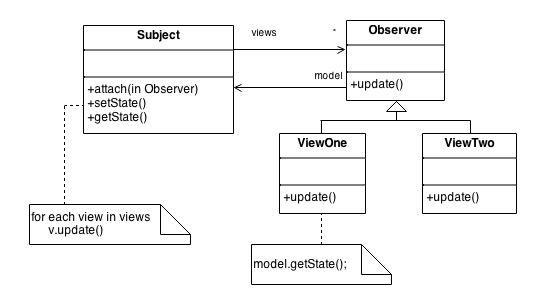
\includegraphics[scale=0.7]{images/observer.jpg}
\caption{UML dijagram obrasca za projektovanje "Posmatrač".} 
\label{fig:UMLObserver}
\end{figure}

Primer upotrebe ovog obrasca može biti aukcija gde je aukcionar subjekat i započinje aukciju, dok učesnici aukcije (objekti) posmatraju aukcionera i reaguju na podizanje cene. Prihvatanje promene cene menja trenutnu cenu i aukcioner oglašava promenu iste, a svi učesnici aukcije dobijaju informaciju da se izmena izvršila. Za potrebe ovog rada, primer upotrebe može biti obilazak stablolike kolekcije (recimo stabla parsiranja) i obaveštavanje o nailasku na čvorove određenih tipova. Te informacije se dalje mogu iskoristiti za izračunavanja nad pomenutom strukturom ili generisanje novih struktura (recimo AST). 

\subsection{Obrazac "Posetilac"}
\label{subsec:DesignPatternsListener}

Obrazac za projektovanje \emph{Posetilac} je strukturni obrazac za projektovanje koji predstavlja operaciju koju je potrebno izvesti nad elementima objektne strukture. Posetilac omogućava definisanje nove operacije bez izmena klasa elemenata nad kojima operiše. Operacija koja će se izvesti zavisi od imena zahteva, tipa posetioca i tipa elementa kog posećuje. Na slici \ref{fig:UMLVisitor} se može videti UML dijagram \cite{UML} ovog obrasca. 

\begin{figure}[h!]
    \centering
    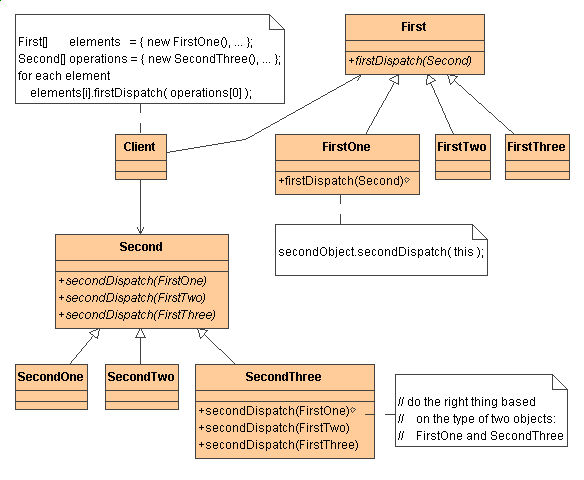
\includegraphics[scale=0.6]{images/visitor.jpg}
    \caption{UML dijagram obrasca za projektovanje "Posetilac".} 
    \label{fig:UMLVisitor}
\end{figure}

Primer upotrebe ovog obrasca može biti operisanje taksi kompanija. Kada osoba pozove taksi kompaniju (prihvatanje posetioca), kompanija šalje vozilo osobi koja je pozvala kompaniju. Nakon ulaska u vozilo (posetilac), mušterija ne kontroliše svoj transport već je to u rukama taksiste (posetioca). Za potrebe ovog rada, primer upotrebe može biti prikupljanje informacija o kolekciji stablolike strukture (recimo stablo parsiranja) i korišćenje istih za neko izračunavanje ili generisanje novih struktura (recimo AST). 
